%==========================================================
% CHAPTER 4: Vektoriai erdvėje
%==========================================================
\chapter{Vektoriai erdvėje}

\section{Vektoriaus sąvoka erdvėje}

Erdvėje, kaip ir plokštumoje, daugelis fizinių dydžių -- jėga, greitis, pagreitis, poslinkis -- 
turi ne tik dydį, bet ir kryptį. Tokiems dydžiams aprašyti naudojama \textbf{vektoriaus} sąvoka.

% -------------------------------------------------------
\subsection{Vektoriaus apibrėžimas}

\begin{definition}[Vektorius erdvėje]
\textbf{Vektorius} $\vec{a}$ erdvėje -- tai nukreiptasis atkarpos atkarpa, turinti 
\textbf{pradžios tašką} (uodegą) ir \textbf{galo tašką} (viršūnę, rodyklę).
Vektorius, kurio pradžios taškas yra $A$, o galo taškas -- $B$, žymimas $\overrightarrow{AB}$.
\end{definition}

\begin{remark}
Vektorius erdvėje skiriasi nuo vektoriaus plokštumoje tuo, kad jo komponentų yra 
\textbf{trys}, o ne dvi. Visi apibrėžimai ir savybės natūraliai išplečiamos iš 
plokštumos į erdvę.
\end{remark}

Vektoriaus geometrinė iliustracija:

\begin{center}
\begin{tikzpicture}[x={({cos(15)*1cm},{sin(15)*1cm})},
                    y={(1cm,0cm)},
                    z={(0cm,1cm)},
                    scale=1.2]
  % koordinačių ašys
  \draw[->, gray] (0,0,0) -- (3,0,0) node[right] {$x$};
  \draw[->, gray] (0,0,0) -- (0,3,0) node[right] {$y$};
  \draw[->, gray] (0,0,0) -- (0,0,3) node[above] {$z$};
  % vektorius
  \draw[->, thick, blue] (0.5,0.5,0.5) -- (2.2,1.8,2.0) 
        node[midway, above left] {$\overrightarrow{AB}$};
  \filldraw[blue] (0.5,0.5,0.5) circle (1.5pt) node[below left] {$A$};
  \filldraw[blue] (2.2,1.8,2.0) circle (1.5pt) node[above right] {$B$};
\end{tikzpicture}
\end{center}

% -------------------------------------------------------
\subsection{Vektoriaus ilgis (modulis)}

\begin{definition}[Vektoriaus ilgis]
\textbf{Vektoriaus ilgis} (arba \textbf{modulis}) $|\vec{a}|$ -- tai atkarpos 
$\overrightarrow{AB}$ ilgis, t.~y. atstumas nuo pradžios taško $A$ iki galo taško $B$.
\end{definition}

Jei vektoriaus koordinatės erdvėje yra $\vec{a} = (x;\, y;\, z)$, tai jo ilgis:
\[
    |\vec{a}| = \sqrt{x^2 + y^2 + z^2}.
\]

\begin{example}
Duotas vektorius $\vec{a} = (2;\,-1;\,3)$. Raskite jo ilgį.\\[4pt]
\textbf{Sprendimas:}
\[
    |\vec{a}| = \sqrt{2^2 + (-1)^2 + 3^2} = \sqrt{4 + 1 + 9} = \sqrt{14}.
\]
\end{example}

% -------------------------------------------------------
\subsection{Specialieji vektoriai}

\begin{definition}[Nulinis vektorius]
\textbf{Nulinis vektorius} $\vec{0}$ -- vektorius, kurio pradžios ir galo taškai sutampa, 
t.~y. $|\vec{0}| = 0$. Nuliniam vektoriui kryptis nėra apibrėžta.
\end{definition}

\begin{definition}[Vienetinis vektorius]
\textbf{Vienetinis vektorius} -- vektorius, kurio ilgis lygus vienetui: $|\vec{e}| = 1$.
\end{definition}

\begin{definition}[Priešingi vektoriai]
Vektoriai $\vec{a}$ ir $\vec{b}$ yra \textbf{priešingi}, jei jie turi tą pačią kryptinę 
tiesę, lygius ilgius, bet \textbf{priešingas kryptis}. Rašoma $\vec{b} = -\vec{a}$.
\end{definition}

% -------------------------------------------------------
\subsection{Lygūs vektoriai}

\begin{definition}[Lygūs vektoriai]
Du vektoriai $\overrightarrow{AB}$ ir $\overrightarrow{CD}$ yra \textbf{lygūs} 
($\overrightarrow{AB} = \overrightarrow{CD}$), jei jie turi:
\begin{enumerate}[label=\arabic*.]
    \item vienodus ilgius: $|\overrightarrow{AB}| = |\overrightarrow{CD}|$,
    \item vienodas kryptis.
\end{enumerate}
\end{definition}

\begin{remark}
Erdvėje vektorius \textbf{nėra susietas} su konkrečia padėtimi -- jis gali būti laisvai 
perkeliamas lygiagrečiai, išlaikant ilgį ir kryptį. Todėl vektoriai vadinami 
\textbf{laisvaisiais vektoriais}.
\end{remark}

% -------------------------------------------------------
\subsection{Kolinerūs ir komplanarūs vektoriai}

\begin{definition}[Kolinerūs vektoriai]
Du vektoriai yra \textbf{kolinerūs} (arba \textbf{lygiagrečiai}), jei jie guli ant tos 
pačios tiesės arba lygiagrečių tiesių. Rašoma $\vec{a} \parallel \vec{b}$.
\end{definition}

\begin{definition}[Komplanarūs vektoriai]
Trys ar daugiau vektorių yra \textbf{komplanarūs}, jei visi jie guli toje pačioje 
plokštumoje arba lygiagrečiose plokštumose.
\end{definition}

\begin{remark}
Bet kurie \textbf{du} vektoriai visada yra komplanarūs (juos visada galima patalpinti į 
vieną bendrą plokštumą). Tačiau trys vektoriai nebūtinai yra komplanarūs.
\end{remark}

\begin{example}
Kubo $ABCDA_1B_1C_1D_1$ kraštinės ilgis yra $1$. Nustatykite, ar vektoriai 
$\overrightarrow{AB}$, $\overrightarrow{AD}$, $\overrightarrow{AA_1}$ yra komplanarūs.\\[4pt]
\textbf{Sprendimas:} Vektorius $\overrightarrow{AB}$ nukreiptas išilgai $x$ ašies, 
$\overrightarrow{AD}$ -- išilgai $y$ ašies, $\overrightarrow{AA_1}$ -- išilgai $z$ ašies. 
Kadangi nė vienas iš jų negali būti išreikštas kitų dviejų tiesine kombinacija, šie trys 
vektoriai \textbf{nėra komplanarūs}.
\end{example}

% -------------------------------------------------------
\subsection{Vektoriaus koordinatės erdvėje}

Erdvėje įvedama stačiakampė koordinačių sistema su \textbf{trimis} statmenomis ašimis: 
$Ox$, $Oy$, $Oz$. Vienetiniai vektoriai šiomis ašimis žymimi $\vec{i}$, $\vec{j}$, 
$\vec{k}$.

\begin{definition}[Vektoriaus koordinatės]
Jei $A = (x_1;\, y_1;\, z_1)$ ir $B = (x_2;\, y_2;\, z_2)$, tai vektoriaus 
$\overrightarrow{AB}$ \textbf{koordinatės}:
\[
    \overrightarrow{AB} = (x_2 - x_1;\; y_2 - y_1;\; z_2 - z_1).
\]
Kiekvienas vektorius $\vec{a} = (x;\, y;\, z)$ gali būti užrašytas per bazinius vektorius:
\[
    \vec{a} = x\,\vec{i} + y\,\vec{j} + z\,\vec{k}.
\]
\end{definition}

\begin{example}
Duoti taškai $A(1;\,-2;\,3)$ ir $B(4;\,0;\,-1)$. Raskite vektoriaus $\overrightarrow{AB}$ 
koordinates ir ilgį.\\[4pt]
\textbf{Sprendimas:}
\[
    \overrightarrow{AB} = (4-1;\; 0-(-2);\; -1-3) = (3;\, 2;\, -4).
\]
\[
    |\overrightarrow{AB}| = \sqrt{3^2 + 2^2 + (-4)^2} = \sqrt{9 + 4 + 16} = \sqrt{29}.
\]
\end{example}

% -------------------------------------------------------
\subsection{Uždaviniai}

\begin{exercise}
Duoti taškai $M(0;\,1;\,-2)$ ir $N(3;\,-1;\,4)$. 
Raskite vektoriaus $\overrightarrow{MN}$ koordinates ir jo ilgį.
\end{exercise}

\begin{exercise}
Ar vektoriai $\vec{a} = (2;\,4;\,-2)$ ir $\vec{b} = (-1;\,-2;\,1)$ yra kolinerūs? 
Pagrįskite atsakymą.
\end{exercise}

\begin{exercise}
Kubo $ABCDA_1B_1C_1D_1$ kraštinės ilgis lygus $a$. Išreikškite vektorių 
$\overrightarrow{AC_1}$ per bazinius vektorius $\vec{i}$, $\vec{j}$, $\vec{k}$ ir 
raskite jo ilgį.
\end{exercise}

\begin{exercise}
Duotas vektorius $\vec{a} = (x;\,2;\,-3)$. Žinoma, kad $|\vec{a}| = \sqrt{17}$. 
Raskite visas galimas $x$ reikšmes.
\end{exercise}


\section{Vektorių veiksmai}

Šiame skyriuje nagrinėsime pagrindinius veiksmus su vektoriais: sudėtį, atimtį ir
daugybą iš skaičiaus. Šie veiksmai sudaro vektorių algebros pagrindą ir plačiai
naudojami geometrijoje, fizikoje bei inžinerijoje.

% ─────────────────────────────────────────────────────────────────────────────
\subsection{Vektorių sudėtis ir atimtis}
% ─────────────────────────────────────────────────────────────────────────────

\subsubsection*{Vektorių suma}

\begin{definition}
Vektorių $\vec{a}$ ir $\vec{b}$ \textbf{suma} – tai vektorius $\vec{c} = \vec{a} + \vec{b}$,
gautas geometriškai taikant \emph{trikampio taisyklę} arba
\emph{lygiagretainio taisyklę}.
\end{definition}

\paragraph{Trikampio taisyklė.}
Nuo bet kurio taško $A$ atidedame vektorių $\overrightarrow{AB} = \vec{a}$.
Nuo taško $B$ atidedame vektorių $\overrightarrow{BC} = \vec{b}$.
Tada $\vec{a} + \vec{b} = \overrightarrow{AC}$.

\begin{center}
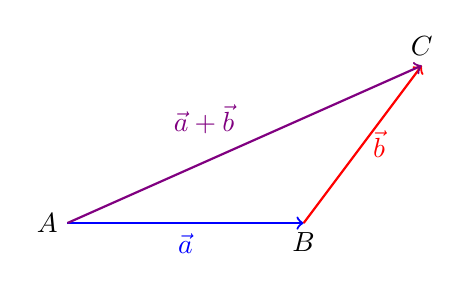
\begin{tikzpicture}
  \coordinate (A) at (0,0);
  \coordinate (B) at (3,0);
  \coordinate (C) at (4.5,2);
  \draw[->, thick, blue]   (A) -- (B) node[midway, below] {$\vec{a}$};
  \draw[->, thick, red]    (B) -- (C) node[midway, right] {$\vec{b}$};
  \draw[->, thick, violet] (A) -- (C) node[midway, above left] {$\vec{a}+\vec{b}$};
  \node[left]  at (A) {$A$};
  \node[below] at (B) {$B$};
  \node[above] at (C) {$C$};
\end{tikzpicture}
\end{center}

\paragraph{Lygiagretainio taisyklė.}
Nuo taško $A$ atidedame abu vektorius $\vec{a}$ ir $\vec{b}$.
Suma $\vec{a} + \vec{b}$ yra lygiagretainio įstrižainė, einanti iš taško $A$.

\begin{center}
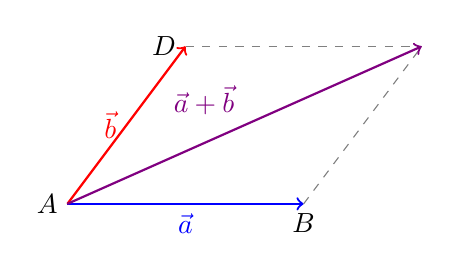
\begin{tikzpicture}
  \coordinate (A) at (0,0);
  \coordinate (B) at (3,0);
  \coordinate (D) at (1.5,2);
  \coordinate (C) at (4.5,2);
  \draw[->, thick, blue]   (A) -- (B) node[midway, below] {$\vec{a}$};
  \draw[->, thick, red]    (A) -- (D) node[midway, left]  {$\vec{b}$};
  \draw[dashed, gray]      (B) -- (C);
  \draw[dashed, gray]      (D) -- (C);
  \draw[->, thick, violet] (A) -- (C) node[midway, above left] {$\vec{a}+\vec{b}$};
  \node[left]  at (A) {$A$};
  \node[below] at (B) {$B$};
  \node[left]  at (D) {$D$};
\end{tikzpicture}
\end{center}

\subsubsection*{Vektorių sudėties savybės}

\begin{theorem}
Vektorių sudėtis turi šias savybes:
\begin{enumerate}[label=\arabic*°]
  \item \textbf{Komutatyvumas:}
        \[
          \vec{a} + \vec{b} = \vec{b} + \vec{a}.
        \]
  \item \textbf{Asociatyvumas:}
        \[
          (\vec{a} + \vec{b}) + \vec{c} = \vec{a} + (\vec{b} + \vec{c}).
        \]
  \item \textbf{Nulinio vektoriaus savybė:}
        \[
          \vec{a} + \vec{0} = \vec{a}.
        \]
  \item \textbf{Priešingo vektoriaus savybė:}
        \[
          \vec{a} + (-\vec{a}) = \vec{0}.
        \]
\end{enumerate}
\end{theorem}

\subsubsection*{Kelių vektorių suma}

Sudedant $n$ vektorių $\vec{a}_1, \vec{a}_2, \ldots, \vec{a}_n$, nuo pirmojo vektoriaus galo
atidedamas antrasis, nuo antrojo – trečiasis ir t.~t. Gautas vektorius, jungiantis pirmojo
vektoriaus pradžią su paskutiniojo vektoriaus galu, yra visų vektorių suma:
\[
  \vec{S} = \vec{a}_1 + \vec{a}_2 + \cdots + \vec{a}_n.
\]

\begin{remark}
Jei vektoriai sudaro uždarą daugiakampį (t.~y. paskutinio vektoriaus galas sutampa su
pirmojo pradžia), tai jų suma lygi nuliniam vektoriui $\vec{0}$.
\end{remark}

\subsubsection*{Vektorių atimtis}

\begin{definition}
Vektorių $\vec{a}$ ir $\vec{b}$ \textbf{skirtumas} – tai vektorius
\[
  \vec{a} - \vec{b} = \vec{a} + (-\vec{b}),
\]
kur $-\vec{b}$ yra $\vec{b}$ priešingas vektorius (to paties ilgio, bet priešingos krypties).
\end{definition}

Geometriškai: jei $\vec{a} = \overrightarrow{OA}$ ir $\vec{b} = \overrightarrow{OB}$ (abu išeinantys
iš vieno taško $O$), tai
\[
  \vec{a} - \vec{b} = \overrightarrow{BA}.
\]

\begin{center}
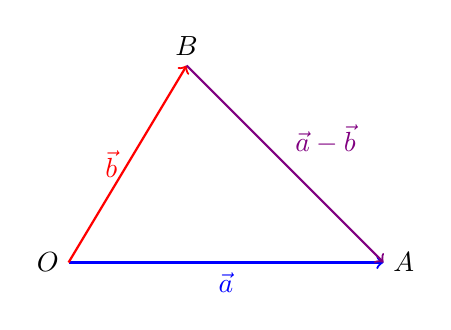
\begin{tikzpicture}
  \coordinate (O) at (0,0);
  \coordinate (A) at (4,0);
  \coordinate (B) at (1.5,2.5);
  \draw[->, thick, blue]   (O) -- (A) node[midway, below] {$\vec{a}$};
  \draw[->, thick, red]    (O) -- (B) node[midway, left]  {$\vec{b}$};
  \draw[->, thick, violet] (B) -- (A) node[midway, above right] {$\vec{a}-\vec{b}$};
  \node[left]  at (O) {$O$};
  \node[right] at (A) {$A$};
  \node[above] at (B) {$B$};
\end{tikzpicture}
\end{center}

\subsubsection*{Veiksmai koordinatėmis}

Jei vektoriai duoti koordinatėmis plokštumoje:
\[
  \vec{a} = (a_1,\, a_2), \qquad \vec{b} = (b_1,\, b_2),
\]
tai:
\[
  \vec{a} + \vec{b} = (a_1 + b_1,\; a_2 + b_2),
\]
\[
  \vec{a} - \vec{b} = (a_1 - b_1,\; a_2 - b_2).
\]

Erdvėje ($\vec{a} = (a_1, a_2, a_3)$, $\vec{b} = (b_1, b_2, b_3)$):
\[
  \vec{a} \pm \vec{b} = (a_1 \pm b_1,\; a_2 \pm b_2,\; a_3 \pm b_3).
\]

\begin{example}
Duoti vektoriai $\vec{a} = (3, -1)$ ir $\vec{b} = (-2, 4)$. Raskite
$\vec{a} + \vec{b}$ ir $\vec{a} - \vec{b}$.

\textbf{Sprendimas:}
\[
  \vec{a} + \vec{b} = (3 + (-2),\; -1 + 4) = (1,\; 3).
\]
\[
  \vec{a} - \vec{b} = (3 - (-2),\; -1 - 4) = (5,\; -5).
\]
\end{example}

\begin{exercise}
Duoti vektoriai $\vec{a} = (2, 5, -3)$ ir $\vec{b} = (-1, 2, 4)$.
Apskaičiuokite $\vec{a} + \vec{b}$, $\vec{a} - \vec{b}$ ir $\vec{b} - \vec{a}$.
\end{exercise}

\begin{exercise}
Taškai $A(1, 2)$, $B(4, -1)$ ir $C(-2, 3)$.
Raskite vektorių $\overrightarrow{AB} + \overrightarrow{BC}$ ir patikrinkite,
ar gautasis vektorius lygus $\overrightarrow{AC}$.
\end{exercise}

% ─────────────────────────────────────────────────────────────────────────────
\subsection{Vektoriaus daugyba iš skaičiaus}
% ─────────────────────────────────────────────────────────────────────────────

\subsubsection*{Apibrėžimas ir geometrinė prasmė}

\begin{definition}
\textbf{Vektoriaus $\vec{a}$ daugyba iš realaus skaičiaus $\lambda$} – tai vektorius
$\lambda\vec{a}$, tenkinantis sąlygas:
\begin{itemize}
  \item $|\lambda\vec{a}| = |\lambda| \cdot |\vec{a}|$ \quad (ilgis padidėja $|\lambda|$ kartų);
  \item jei $\lambda > 0$, vektorius $\lambda\vec{a}$ yra \emph{tos pačios krypties} kaip $\vec{a}$;
  \item jei $\lambda < 0$, vektorius $\lambda\vec{a}$ yra \emph{priešingos krypties} kaip $\vec{a}$;
  \item jei $\lambda = 0$ arba $\vec{a} = \vec{0}$, tai $\lambda\vec{a} = \vec{0}$.
\end{itemize}
\end{definition}

\begin{center}
\begin{tikzpicture}
  \draw[->, thick, blue]   (0,1.5)   -- (3,1.5)   node[right] {$\vec{a}$};
  \draw[->, thick, teal]   (0,0.5)   -- (4.5,0.5) node[right] {$1{,}5\,\vec{a}$};
  \draw[->, thick, orange] (0,-0.5)  -- (1.5,-0.5) node[right] {$0{,}5\,\vec{a}$};
  \draw[->, thick, red]    (3,-1.5)  -- (0,-1.5)  node[left]  {$-\vec{a}$};
\end{tikzpicture}
\end{center}

\subsubsection*{Daugybos iš skaičiaus savybės}

\begin{theorem}
Tebūnie $\vec{a}$, $\vec{b}$ – bet kurie vektoriai, o $\lambda$, $\mu \in \mathbb{R}$.
Tada galioja:
\begin{enumerate}[label=\arabic*°]
  \item \textbf{Asociatyvumas su skaičiais:}
        \[
          \lambda(\mu\vec{a}) = (\lambda\mu)\vec{a}.
        \]
  \item \textbf{Distributyvumas dėl vektorių sumos:}
        \[
          \lambda(\vec{a} + \vec{b}) = \lambda\vec{a} + \lambda\vec{b}.
        \]
  \item \textbf{Distributyvumas dėl skaičių sumos:}
        \[
          (\lambda + \mu)\vec{a} = \lambda\vec{a} + \mu\vec{a}.
        \]
  \item \textbf{Vieneto savybė:}
        \[
          1 \cdot \vec{a} = \vec{a}.
        \]
\end{enumerate}
\end{theorem}

\subsubsection*{Vektoriaus daugyba iš skaičiaus koordinatėmis}

Jei $\vec{a} = (a_1, a_2)$ plokštumoje, tai:
\[
  \lambda\vec{a} = (\lambda a_1,\; \lambda a_2).
\]

Erdvėje, jei $\vec{a} = (a_1, a_2, a_3)$:
\[
  \lambda\vec{a} = (\lambda a_1,\; \lambda a_2,\; \lambda a_3).
\]

\begin{example}
Duotas vektorius $\vec{a} = (2, -3)$. Raskite $3\vec{a}$ ir $-2\vec{a}$.

\textbf{Sprendimas:}
\[
  3\vec{a} = (3 \cdot 2,\; 3 \cdot (-3)) = (6,\; -9).
\]
\[
  -2\vec{a} = (-2 \cdot 2,\; -2 \cdot (-3)) = (-4,\; 6).
\]
\end{example}

\subsubsection*{Kolinearieji vektoriai}

\begin{definition}
Vektoriai $\vec{a}$ ir $\vec{b}$ vadinami \textbf{kolineariais} (lygiagretais), jei egzistuoja
toks realus skaičius $\lambda$, kad:
\[
  \vec{b} = \lambda\vec{a} \quad (\vec{a} \ne \vec{0}).
\]
\end{definition}

\begin{remark}
Koordinatėmis: vektoriai $\vec{a} = (a_1, a_2)$ ir $\vec{b} = (b_1, b_2)$ yra kolinearūs
tada ir tik tada, kai
\[
  a_1 b_2 - a_2 b_1 = 0.
\]
\end{remark}

\subsubsection*{Vienetinis vektorius}

\begin{definition}
\textbf{Vienetiniu vektoriumi} (arba \emph{ortu}) vadinamas vektorius, kurio ilgis lygus 1.
Vektoriaus $\vec{a} \ne \vec{0}$ ortas žymimas $\vec{a}^{\,0}$ ir apskaičiuojamas:
\[
  \vec{a}^{\,0} = \frac{\vec{a}}{|\vec{a}|} = \frac{1}{|\vec{a}|}\,\vec{a}.
\]
\end{definition}

\begin{example}
Raskite vektoriaus $\vec{a} = (3, 4)$ ortą.

\textbf{Sprendimas:}
\[
  |\vec{a}| = \sqrt{3^2 + 4^2} = \sqrt{9 + 16} = \sqrt{25} = 5.
\]
\[
  \vec{a}^{\,0} = \frac{1}{5}(3, 4) = \left(\frac{3}{5},\; \frac{4}{5}\right).
\]
\textbf{Patikrinimas:} $\left|\vec{a}^{\,0}\right| = \sqrt{\left(\tfrac{3}{5}\right)^2 + \left(\tfrac{4}{5}\right)^2} = \sqrt{\tfrac{9}{25}+\tfrac{16}{25}} = 1$. \checkmark
\end{example}

\subsubsection*{Sudėtingesni pavyzdžiai}

\begin{example}
Duoti vektoriai $\vec{a} = (1, -2)$ ir $\vec{b} = (3, 1)$. Apskaičiuokite $2\vec{a} - 3\vec{b}$.

\textbf{Sprendimas:}
\begin{align*}
  2\vec{a} - 3\vec{b}
    &= 2(1, -2) - 3(3, 1) \\
    &= (2, -4) - (9, 3) \\
    &= (2 - 9,\; -4 - 3) \\
    &= (-7,\; -7).
\end{align*}
\end{example}

\begin{exercise}
Duoti vektoriai $\vec{a} = (-1, 3, 2)$ ir $\vec{b} = (2, -1, 4)$.
Raskite $4\vec{a} - 2\vec{b}$ ir šio rezultato ilgį.
\end{exercise}

\begin{exercise}
Ar vektoriai $\vec{a} = (2, -4)$ ir $\vec{b} = (-3, 6)$ yra kolinearūs? Pagrįskite.
\end{exercise}

\begin{tcolorbox}[title={Pagrindinės formulės}, colback=blue!5, colframe=blue!50]
\begin{align*}
  \vec{a} + \vec{b} &= (a_1 + b_1,\; a_2 + b_2) \\[4pt]
  \vec{a} - \vec{b} &= (a_1 - b_1,\; a_2 - b_2) \\[4pt]
  \lambda\vec{a}    &= (\lambda a_1,\; \lambda a_2) \\[4pt]
  \vec{a}^{\,0}     &= \dfrac{\vec{a}}{|\vec{a}|} \\[4pt]
  \vec{a} \parallel \vec{b} &\iff a_1 b_2 - a_2 b_1 = 0
\end{align*}
\end{tcolorbox}


\section{Skaliarinė sandauga}

Skaliarinė sandauga yra viena svarbiausių vektorių algebros operacijų, jungianti geometrinę ir algebrinę vektorių interpretaciją. Ji plačiai taikoma fizikoje, inžinerijoje ir matematikoje – apskaičiuojant darbą, kampus, projekcijas ir kt.

\begin{definition}
Dviejų nenulinių vektorių $\vec{a}$ ir $\vec{b}$ \textbf{skaliarine sandauga} vadinamas skaičius, lygus šių vektorių ilgių ir kampo tarp jų kosinuso sandaugai:
\[
\vec{a} \cdot \vec{b} = |\vec{a}| \cdot |\vec{b}| \cdot \cos\varphi,
\]
kur $\varphi$ -- kampas tarp vektorių $\vec{a}$ ir $\vec{b}$, $0^\circ \leq \varphi \leq 180^\circ$.

Jei bent vienas iš vektorių yra nulinis, tai $\vec{a} \cdot \vec{b} = 0$.
\end{definition}

\begin{remark}
Skaliarinės sandaugos rezultatas yra \textbf{skaičius} (skaliaras), o ne vektorius -- tai ir lemia pavadinimą ,,skaliarinė''.
\end{remark}

\subsection{Skaliarinės sandaugos savybės}

Skaliarinė sandauga turi kelias pagrindines algebrines savybes, analogiškas įprastinei skaičių daugybai.

\begin{theorem}[Skaliarinės sandaugos savybės]
Tebūnie $\vec{a}$, $\vec{b}$, $\vec{c}$ -- bet kokie vektoriai, o $\lambda \in \mathbb{R}$ -- realusis skaičius. Tada:
\begin{enumerate}[label=\arabic*.]
    \item \textbf{Komutatyvumas:}
    \[
    \vec{a} \cdot \vec{b} = \vec{b} \cdot \vec{a}.
    \]
    \item \textbf{Distributyvumas dėl sudėties:}
    \[
    \vec{a} \cdot (\vec{b} + \vec{c}) = \vec{a} \cdot \vec{b} + \vec{a} \cdot \vec{c}.
    \]
    \item \textbf{Asociatyvumas su skaičiumi:}
    \[
    (\lambda \vec{a}) \cdot \vec{b} = \lambda (\vec{a} \cdot \vec{b}).
    \]
    \item \textbf{Sandauga su pačiu savimi (kvadratas):}
    \[
    \vec{a} \cdot \vec{a} = |\vec{a}|^2 \geq 0, \quad \text{ir} \quad \vec{a} \cdot \vec{a} = 0 \iff \vec{a} = \vec{0}.
    \]
\end{enumerate}
\end{theorem}

\begin{remark}
Skaliarinė sandauga \textbf{nėra asociatyvi}: reiškinys $(\vec{a} \cdot \vec{b}) \cdot \vec{c}$ netenka prasmės, nes $\vec{a} \cdot \vec{b}$ yra skaičius, o ne vektorius.
\end{remark}

\subsubsection*{Svarbiausios pasekmės}

\begin{corollary}[Statmenumas]
Du nenuliniai vektoriai $\vec{a}$ ir $\vec{b}$ yra \textbf{statmeni} ($\vec{a} \perp \vec{b}$) tada ir tik tada, kai
\[
\vec{a} \cdot \vec{b} = 0.
\]
\end{corollary}

\begin{proof}
Jei $\vec{a} \perp \vec{b}$, tai $\varphi = 90^\circ$, todėl $\cos 90^\circ = 0$ ir $\vec{a} \cdot \vec{b} = |\vec{a}| \cdot |\vec{b}| \cdot 0 = 0$.
Atvirkščiai, jei $\vec{a} \cdot \vec{b} = 0$ ir $|\vec{a}| \neq 0$, $|\vec{b}| \neq 0$, tai $\cos\varphi = 0$, vadinasi $\varphi = 90^\circ$.
\end{proof}

\begin{corollary}[Kolinearumas]
Jei vektoriai $\vec{a}$ ir $\vec{b}$ yra \textbf{vienakrypčiai} ($\varphi = 0^\circ$), tai
\[
\vec{a} \cdot \vec{b} = |\vec{a}| \cdot |\vec{b}|.
\]
Jei jie \textbf{priešingakrypčiai} ($\varphi = 180^\circ$), tai
\[
\vec{a} \cdot \vec{b} = -|\vec{a}| \cdot |\vec{b}|.
\]
\end{corollary}

\subsubsection*{Skaliarinė sandauga koordinatėmis}

Plokštumoje, jei $\vec{a} = (a_1,\, a_2)$ ir $\vec{b} = (b_1,\, b_2)$, tai:
\[
\vec{a} \cdot \vec{b} = a_1 b_1 + a_2 b_2.
\]

Erdvėje, jei $\vec{a} = (a_1,\, a_2,\, a_3)$ ir $\vec{b} = (b_1,\, b_2,\, b_3)$, tai:
\[
\vec{a} \cdot \vec{b} = a_1 b_1 + a_2 b_2 + a_3 b_3.
\]

\begin{remark}
Iš šios formulės išplaukia patogi vektoriaus ilgio skaičiavimo formulė:
\[
|\vec{a}| = \sqrt{\vec{a} \cdot \vec{a}} = \sqrt{a_1^2 + a_2^2}
\]
plokštumoje, arba $|\vec{a}| = \sqrt{a_1^2 + a_2^2 + a_3^2}$ erdvėje.
\end{remark}

\begin{example}
Duoti vektoriai $\vec{a} = (3,\, -1)$ ir $\vec{b} = (2,\, 6)$. Apskaičiuokite $\vec{a} \cdot \vec{b}$ ir nustatykite, ar vektoriai statmeni.

\textbf{Sprendimas:}
\[
\vec{a} \cdot \vec{b} = 3 \cdot 2 + (-1) \cdot 6 = 6 - 6 = 0.
\]
Kadangi $\vec{a} \cdot \vec{b} = 0$, vektoriai $\vec{a}$ ir $\vec{b}$ yra \textbf{statmeni}.
\end{example}

\begin{example}
Taikant distributyvumo savybę, supaprastinkite: $(\vec{a} + \vec{b})^2$.

\textbf{Sprendimas:}
\begin{align*}
(\vec{a} + \vec{b})^2 &= (\vec{a} + \vec{b}) \cdot (\vec{a} + \vec{b}) \\
&= \vec{a} \cdot \vec{a} + \vec{a} \cdot \vec{b} + \vec{b} \cdot \vec{a} + \vec{b} \cdot \vec{b} \\
&= |\vec{a}|^2 + 2(\vec{a} \cdot \vec{b}) + |\vec{b}|^2.
\end{align*}
\end{example}

\begin{exercise}
Duoti vektoriai $\vec{a} = (1,\, 2,\, -2)$ ir $\vec{b} = (-3,\, 0,\, 4)$.
\begin{enumerate}[label=\alph*)]
    \item Apskaičiuokite $\vec{a} \cdot \vec{b}$.
    \item Apskaičiuokite $|\vec{a}|$ ir $|\vec{b}|$.
    \item Apskaičiuokite $(\vec{a} - \vec{b}) \cdot \vec{a}$.
\end{enumerate}
\end{exercise}

\subsection{Kampo tarp vektorių skaičiavimas}

Žinodami skaliarinę sandaugą koordinatėmis ir jos ryšį su kampu, galime apskaičiuoti kampą tarp bet kurių dviejų nenulinių vektorių.

\subsubsection*{Pagrindinė formulė}

Iš skaliarinės sandaugos apibrėžimo:
\[
\vec{a} \cdot \vec{b} = |\vec{a}| \cdot |\vec{b}| \cdot \cos\varphi
\]
išreiškiame $\cos\varphi$:

\begin{tcolorbox}[colback=blue!5!white, colframe=blue!60!black, title=Kampo tarp vektorių formulė]
\[
\cos\varphi = \frac{\vec{a} \cdot \vec{b}}{|\vec{a}| \cdot |\vec{b}|},
\]
kur $0^\circ \leq \varphi \leq 180^\circ$.

Koordinatėmis (plokštuma):
\[
\cos\varphi = \frac{a_1 b_1 + a_2 b_2}{\sqrt{a_1^2 + a_2^2} \cdot \sqrt{b_1^2 + b_2^2}}.
\]

Koordinatėmis (erdvė):
\[
\cos\varphi = \frac{a_1 b_1 + a_2 b_2 + a_3 b_3}{\sqrt{a_1^2 + a_2^2 + a_3^2} \cdot \sqrt{b_1^2 + b_2^2 + b_3^2}}.
\]
\end{tcolorbox}

\subsubsection*{Kampo ženklo interpretacija}

Remdamiesi kosinuso reikšme, galime nustatyti kampo tipą:

\begin{center}
\begin{tabular}{|c|c|c|}
\hline
\textbf{Sąlyga} & \textbf{Kampas} $\varphi$ & \textbf{Geometrinė prasmė} \\
\hline
$\vec{a} \cdot \vec{b} > 0$ & $0^\circ < \varphi < 90^\circ$ & Ūmus kampas \\
\hline
$\vec{a} \cdot \vec{b} = 0$ & $\varphi = 90^\circ$ & Stačias kampas \\
\hline
$\vec{a} \cdot \vec{b} < 0$ & $90^\circ < \varphi < 180^\circ$ & Bukas kampas \\
\hline
$\vec{a} \cdot \vec{b} = |\vec{a}||\vec{b}|$ & $\varphi = 0^\circ$ & Vienakrypčiai vektoriai \\
\hline
$\vec{a} \cdot \vec{b} = -|\vec{a}||\vec{b}|$ & $\varphi = 180^\circ$ & Priešingakrypčiai vektoriai \\
\hline
\end{tabular}
\end{center}

\begin{example}
Raskite kampą tarp vektorių $\vec{a} = (1,\, \sqrt{3})$ ir $\vec{b} = (\sqrt{3},\, 1)$.

\textbf{Sprendimas:}
\[
\vec{a} \cdot \vec{b} = 1 \cdot \sqrt{3} + \sqrt{3} \cdot 1 = 2\sqrt{3}.
\]
\[
|\vec{a}| = \sqrt{1^2 + (\sqrt{3})^2} = \sqrt{1 + 3} = 2, \quad
|\vec{b}| = \sqrt{(\sqrt{3})^2 + 1^2} = \sqrt{3 + 1} = 2.
\]
\[
\cos\varphi = \frac{2\sqrt{3}}{2 \cdot 2} = \frac{2\sqrt{3}}{4} = \frac{\sqrt{3}}{2}.
\]
\[
\varphi = \arccos\frac{\sqrt{3}}{2} = 30^\circ.
\]
\textbf{Atsakymas:} kampas tarp vektorių lygus $30^\circ$.
\end{example}

\begin{example}
Duoti vektoriai $\vec{u} = (2,\, 1,\, -1)$ ir $\vec{v} = (1,\, -1,\, 2)$. Raskite kampą tarp jų.

\textbf{Sprendimas:}
\[
\vec{u} \cdot \vec{v} = 2 \cdot 1 + 1 \cdot (-1) + (-1) \cdot 2 = 2 - 1 - 2 = -1.
\]
\[
|\vec{u}| = \sqrt{4 + 1 + 1} = \sqrt{6}, \quad |\vec{v}| = \sqrt{1 + 1 + 4} = \sqrt{6}.
\]
\[
\cos\varphi = \frac{-1}{\sqrt{6} \cdot \sqrt{6}} = \frac{-1}{6}.
\]
\[
\varphi = \arccos\!\left(-\frac{1}{6}\right) \approx 99{,}6^\circ.
\]
\textbf{Atsakymas:} kampas tarp vektorių yra bukas, $\varphi \approx 99{,}6^\circ$.
\end{example}

\begin{example}[VBE tipo uždavinys]
Trikampio $ABC$ viršūnių koordinatės: $A(1,\, 2)$, $B(4,\, 6)$, $C(5,\, 2)$. Raskite kampą $\angle BAC$.

\textbf{Sprendimas:}

Sudarome vektorius iš viršūnės $A$:
\[
\vec{AB} = (4-1,\; 6-2) = (3,\, 4), \quad \vec{AC} = (5-1,\; 2-2) = (4,\, 0).
\]
\[
\vec{AB} \cdot \vec{AC} = 3 \cdot 4 + 4 \cdot 0 = 12.
\]
\[
|\vec{AB}| = \sqrt{9 + 16} = 5, \quad |\vec{AC}| = \sqrt{16 + 0} = 4.
\]
\[
\cos(\angle BAC) = \frac{12}{5 \cdot 4} = \frac{12}{20} = \frac{3}{5} = 0{,}6.
\]
\[
\angle BAC = \arccos 0{,}6 \approx 53{,}1^\circ.
\]
\end{example}

\begin{exercise}
\begin{enumerate}[label=\arabic*.]
    \item Raskite kampą tarp vektorių $\vec{a} = (3,\, 4)$ ir $\vec{b} = (-4,\, 3)$.
    \item Vektoriaus $\vec{a} = (x,\, 1)$ ir $\vec{b} = (2,\, -1)$ kampas lygus $90^\circ$. Raskite $x$.
    \item Keturkampio viršūnės: $A(0,0)$, $B(4,0)$, $C(3,3)$, $D(0,3)$. Ar tiesės $AC$ ir $BD$ yra statmenos?
    \item Raskite kampą tarp vektorių $\vec{p} = (2,\, -1,\, 2)$ ir $\vec{q} = (1,\, 2,\, 0)$.
\end{enumerate}
\end{exercise}

\subsubsection*{Projekcija ant vektoriaus}

Susijusi sąvoka -- vektoriaus $\vec{a}$ \textbf{projekcija} kryptimi $\vec{b}$:
\[
\text{pr}_{\vec{b}}\, \vec{a} = \frac{\vec{a} \cdot \vec{b}}{|\vec{b}|} = |\vec{a}| \cos\varphi.
\]
Ši formulė naudinga fizikoje (pvz., apskaičiuojant atliktą darbą: $A = \vec{F} \cdot \vec{s} = |\vec{F}| \cdot |\vec{s}| \cdot \cos\varphi$).


\section{Kolinearūs ir komplanarūs vektoriai}

\subsection{Kolinearūs vektoriai}

\begin{definition}
Du nenuliniai vektoriai vadinami \textbf{kolineariais}, jeigu jie guli vienoje tiesėje arba lygiagretėse tiesėse. Kitaip tariant, kolinearūs vektoriai yra lygiagretūs vienas kitam.
\end{definition}

Kolinearūs vektoriai skirstomi į dvi grupes:
\begin{itemize}
    \item \textbf{Vienkrypčiai} – nukreipti ta pačia kryptimi;
    \item \textbf{Priešpriešiniai} – nukreipti priešingomis kryptimis.
\end{itemize}

\begin{tcolorbox}[colback=blue!5!white, colframe=blue!60!black, title=Kolinearumo požymis]
Du vektoriai $\vec{a}$ ir $\vec{b}$ yra kolinearūs tada ir tik tada, kai egzistuoja toks realusis skaičius $k$, kad
\[
\vec{b} = k\,\vec{a}.
\]
Jei $k > 0$, vektoriai yra vienkrypčiai; jei $k < 0$ – priešpriešiniai.
\end{tcolorbox}

\subsubsection{Kolinearumo sąlyga koordinatėmis}

\paragraph{Plokštumoje.}
Tarkime, $\vec{a} = (x_1,\, y_1)$ ir $\vec{b} = (x_2,\, y_2)$. Vektoriai $\vec{a}$ ir $\vec{b}$ yra kolinearūs tada ir tik tada, kai
\[
x_1 y_2 - x_2 y_1 = 0,
\]
arba, jei $x_2 \neq 0$ ir $y_2 \neq 0$:
\[
\frac{x_1}{x_2} = \frac{y_1}{y_2}.
\]

\paragraph{Erdvėje.}
Tarkime, $\vec{a} = (x_1,\, y_1,\, z_1)$ ir $\vec{b} = (x_2,\, y_2,\, z_2)$. Vektoriai yra kolinearūs tada ir tik tada, kai jų koordinatės proporcingos:
\[
\frac{x_1}{x_2} = \frac{y_1}{y_2} = \frac{z_1}{z_2}.
\]

\begin{remark}
Jei viena iš koordinačių lygi nuliui, atitinkama kitos vektoriaus koordinatė taip pat turi būti lygi nuliui.
\end{remark}

\begin{example}
Nustatykite, ar vektoriai $\vec{a} = (2,\, -4,\, 6)$ ir $\vec{b} = (-1,\, 2,\, -3)$ yra kolinearūs.

\textbf{Sprendimas.} Tikriname proporcingumą:
\[
\frac{2}{-1} = -2, \quad \frac{-4}{2} = -2, \quad \frac{6}{-3} = -2.
\]
Kadangi visos trys santykiai lygūs $-2$, vektoriai yra kolinearūs (priešpriešiniai), nes $\vec{b} = -2\,\vec{a}$.
\end{example}

\begin{example}
Raskite $t$ reikšmę, kuriai esant vektoriai $\vec{a} = (3,\, t,\, -6)$ ir $\vec{b} = (-1,\, 2,\, 2)$ yra kolinearūs.

\textbf{Sprendimas.} Iš kolinearumo sąlygos:
\[
\frac{3}{-1} = \frac{t}{2} = \frac{-6}{2}.
\]
\[
\frac{3}{-1} = -3 \quad \text{ir} \quad \frac{-6}{2} = -3.
\]
Taigi $k = -3$ ir $\frac{t}{2} = -3 \Rightarrow t = -6$.
\end{example}

\begin{exercise}
Ar vektoriai $\vec{a} = (4,\, -2,\, 8)$ ir $\vec{b} = (-2,\, 1,\, -4)$ yra kolinearūs? Jei taip, nurodykite, ar jie vienkrypčiai, ar priešpriešiniai.
\end{exercise}

\begin{exercise}
Raskite $\lambda$ reikšmę, kuriai esant vektoriai $\vec{u} = (\lambda,\, 3,\, -2)$ ir $\vec{v} = (4,\, 6,\, -4)$ yra kolinearūs.
\end{exercise}

% --------------------------------------------------------
\subsection{Komplanarūs vektoriai}

\begin{definition}
Trys ar daugiau vektorių vadinami \textbf{komplanariais}, jeigu juos galima perkelti taip (išlaikant kryptis), kad jie visi gulėtų vienoje plokštumoje.
\end{definition}

Akivaizdu, kad bet kurie \emph{du} vektoriai visada yra komplanarūs – jie apibrėžia bent vieną plokštumą. Todėl komplanarumo sąvoka yra prasminga tik kalbant apie \emph{tris ar daugiau} vektorių.

\begin{tcolorbox}[colback=green!5!white, colframe=green!60!black, title=Komplanarūmo požymis (trijų vektorių)]
Trys vektoriai $\vec{a}$, $\vec{b}$, $\vec{c}$ yra komplanarūs tada ir tik tada, kai jų \textbf{mišrioji sandauga} lygi nuliui:
\[
(\vec{a},\, \vec{b},\, \vec{c}) = \vec{a} \cdot (\vec{b} \times \vec{c}) = 0.
\]
\end{tcolorbox}

\subsubsection{Komplanarūmo sąlyga koordinatėmis}

Tegu $\vec{a} = (a_1,\, a_2,\, a_3)$, $\vec{b} = (b_1,\, b_2,\, b_3)$, $\vec{c} = (c_1,\, c_2,\, c_3)$. Tada vektoriai yra komplanarūs, jei ir tik jei determinantas lygus nuliui:
\[
\begin{vmatrix}
a_1 & a_2 & a_3 \\
b_1 & b_2 & b_3 \\
c_1 & c_2 & c_3
\end{vmatrix} = 0.
\]

\subsubsection{Linijinės kombinacijos kriterijus}

Kitas būdas patikrinti komplanarumą: vektoriai $\vec{a}$, $\vec{b}$, $\vec{c}$ yra komplanarūs tada ir tik tada, kai $\vec{c}$ galima išreikšti kaip $\vec{a}$ ir $\vec{b}$ linijinę kombinaciją, t.~y. egzistuoja tokie skaliarai $x,\, y$, kad:
\[
\vec{c} = x\,\vec{a} + y\,\vec{b}.
\]

\begin{example}
Patikrinkite, ar vektoriai $\vec{a} = (1,\, 2,\, -1)$, $\vec{b} = (0,\, 1,\, 3)$, $\vec{c} = (2,\, 5,\, 1)$ yra komplanarūs.

\textbf{Sprendimas.} Skaičiuojame determinantą:
\[
\begin{vmatrix}
1 & 2 & -1 \\
0 & 1 & 3 \\
2 & 5 & 1
\end{vmatrix}
= 1\cdot(1\cdot1 - 3\cdot5) - 2\cdot(0\cdot1 - 3\cdot2) + (-1)\cdot(0\cdot5 - 1\cdot2).
\]
\[
= 1\cdot(1 - 15) - 2\cdot(0 - 6) + (-1)\cdot(0 - 2)
= 1\cdot(-14) - 2\cdot(-6) + (-1)\cdot(-2)
\]
\[
= -14 + 12 + 2 = 0.
\]
Kadangi determinantas lygus nuliui, vektoriai \textbf{yra komplanarūs}.
\end{example}

\begin{example}
Ar vektoriai $\vec{a} = (1,\, 0,\, 1)$, $\vec{b} = (2,\, 1,\, 0)$, $\vec{c} = (1,\, 1,\, 1)$ yra komplanarūs?

\textbf{Sprendimas.}
\[
\begin{vmatrix}
1 & 0 & 1 \\
2 & 1 & 0 \\
1 & 1 & 1
\end{vmatrix}
= 1\cdot(1\cdot1 - 0\cdot1) - 0\cdot(2\cdot1 - 0\cdot1) + 1\cdot(2\cdot1 - 1\cdot1)
\]
\[
= 1\cdot1 - 0 + 1\cdot1 = 1 + 1 = 2 \neq 0.
\]
Vektoriai \textbf{nėra komplanarūs}.
\end{example}

\begin{exercise}
Nustatykite, kuriai $\lambda$ reikšmei vektoriai $\vec{a} = (1,\, 2,\, 3)$, $\vec{b} = (2,\, \lambda,\, 1)$, $\vec{c} = (3,\, 4,\, 1)$ yra komplanarūs.
\end{exercise}

\begin{exercise}
Patikrinkite, ar vektoriai $\vec{a} = (1,\, -1,\, 2)$, $\vec{b} = (2,\, 0,\, 3)$, $\vec{c} = (3,\, -1,\, 5)$ yra komplanarūs.
\end{exercise}

% --------------------------------------------------------
\subsection{Bazė ir vektorių išreiškimas}

\begin{definition}
Trys vektoriai $\vec{e}_1$, $\vec{e}_2$, $\vec{e}_3$ sudaro \textbf{erdvės bazę}, jei jie yra nekomplanarūs. Bet kokį erdvės vektorių $\vec{v}$ galima vienareikšmiškai išreikšti per bazės vektorius:
\[
\vec{v} = \alpha_1\,\vec{e}_1 + \alpha_2\,\vec{e}_2 + \alpha_3\,\vec{e}_3.
\]
\end{definition}

Standartinė ortonormuota bazė Dekarto koordinačių sistemoje yra $\vec{i} = (1,0,0)$, $\vec{j} = (0,1,0)$, $\vec{k} = (0,0,1)$. Šie vektoriai yra nekomplanarūs, todėl bet kurį erdvės vektorių galima vienareikšmiškai išreikšti per juos.

\begin{tcolorbox}[colback=yellow!5!white, colframe=orange!80!black, title=Apibendrinimas]
\begin{itemize}
    \item \textbf{Kolinearūs vektoriai} – lygiagretūs (guli vienoje ar lygiagretėse tiesėse); $\vec{b} = k\vec{a}$.
    \item \textbf{Komplanarūs vektoriai} – guli vienoje plokštumoje; mišrioji sandauga $(\vec{a}, \vec{b}, \vec{c}) = 0$.
    \item Bet kurie du vektoriai visada yra komplanarūs.
    \item Trys nekomplanarūs vektoriai sudaro erdvės bazę.
\end{itemize}
\end{tcolorbox}

